% ICLR 2026 FinAI Workshop Paper
% Table-Aware Retrieval and Learned Routing for Financial RAG
%
% Compile with: pdflatex main.tex && bibtex main && pdflatex main.tex && pdflatex main.tex

\documentclass{article}

% ============================================================================
% PACKAGES
% ============================================================================
\usepackage[utf8]{inputenc}
\usepackage[T1]{fontenc}
\usepackage{hyperref}
\usepackage{url}
\usepackage{booktabs}
\usepackage{amsfonts}
\usepackage{amsmath}
\usepackage{amssymb}
\usepackage{nicefrac}
\usepackage{microtype}
\usepackage{graphicx}
\usepackage{xcolor}
\usepackage{subcaption}
\usepackage{algorithm}
\usepackage{algorithmic}
\usepackage{multirow}
\usepackage{tikz}
\usepackage{pgfplots}
\pgfplotsset{compat=1.17}
\usetikzlibrary{shapes,arrows,positioning,fit,backgrounds,calc}

% Page layout (approximate ICLR style)
\usepackage[margin=1in]{geometry}

% Colors for the paper
\definecolor{primaryblue}{RGB}{0, 84, 147}
\definecolor{accentgreen}{RGB}{34, 139, 34}
\definecolor{highlightyellow}{RGB}{255, 223, 128}
\definecolor{errorred}{RGB}{178, 34, 34}

% Hyperref setup
\hypersetup{
    colorlinks=true,
    linkcolor=primaryblue,
    citecolor=primaryblue,
    urlcolor=primaryblue
}

% Custom commands
\newcommand{\method}{\textsc{TableRouter}}
\newcommand{\baseline}{\textsc{Baseline}}
\newcommand{\docling}{\textsc{Docling}}
\newcommand{\financebench}{\textsc{FinanceBench}}
\newcommand{\ie}{\textit{i.e.}}
\newcommand{\eg}{\textit{e.g.}}
\newcommand{\etc}{\textit{etc.}}
\newcommand{\vs}{\textit{vs.}}

% Highlight box for key findings
\newcommand{\keybox}[1]{%
    \begin{center}
    \fcolorbox{primaryblue}{highlightyellow!30}{%
        \parbox{0.9\linewidth}{\centering\textbf{Key Finding:} #1}%
    }
    \end{center}
}

% ============================================================================
% DOCUMENT
% ============================================================================
\begin{document}

% ----------------------------------------------------------------------------
% TITLE
% ----------------------------------------------------------------------------
\begin{center}
{\LARGE \textbf{Table-Aware Retrieval and Learned Routing\\[0.3em] for Financial Question Answering}}

\vspace{1em}

{\large
Hanson Xiong\textsuperscript{1} \quad
Junjie Xiong\textsuperscript{1} \quad
[Additional Authors]\textsuperscript{1,2}
}

\vspace{0.5em}

{\normalsize
\textsuperscript{1}University [Affiliation] \quad
\textsuperscript{2}[Second Affiliation]
}

\vspace{0.5em}

{\small \texttt{\{hanson.xiong, junjie.xiong\}@university.edu}}

\vspace{1.5em}

\textit{ICLR 2026 Workshop on Financial AI}
\end{center}

\vspace{1em}

% ----------------------------------------------------------------------------
% ABSTRACT
% ----------------------------------------------------------------------------
\begin{abstract}
Retrieval-Augmented Generation (RAG) systems struggle with financial documents containing complex tables, achieving only 27\% accuracy on numerical extraction tasks. We identify \textbf{table fragmentation during chunking} as the primary bottleneck---not model capability. Our analysis shows that four state-of-the-art LLMs (GPT-4o-mini, Llama 3.1 70B, Qwen 2.5 72B, Llama 3.3 70B) all hit the same $\sim$28\% ceiling on metrics-generated questions, proving the retrieval layer is the constraint.

We present two contributions: (1) \textbf{Table-aware chunking} using Docling with TableFormer achieves 97.9\% table extraction accuracy and improves metrics questions by \textbf{+94\%} (27\%$\rightarrow$52\%); (2) \textbf{Learned pipeline routing} trains a classifier on 21 question features to predict the optimal retrieval configuration per query, eliminating the need to run multiple pipelines.

On the \financebench{} benchmark (150 financial QA pairs), our approach improves overall accuracy from 48.5\% to 60.4\% (+24.5\%), with the largest gains on table-dependent questions. Our router achieves [X]\% accuracy in predicting the optimal pipeline, reducing inference cost by 6$\times$ compared to exhaustive search.
\end{abstract}

% ----------------------------------------------------------------------------
% 1. INTRODUCTION
% ----------------------------------------------------------------------------
\section{Introduction}
\label{sec:introduction}

Financial AI assistants must answer precise numerical questions from complex documents---10-K filings, earnings reports, and regulatory disclosures. Questions like ``\textit{What was Apple's FY2023 operating margin?}'' require extracting exact figures from tables spanning multiple pages. Retrieval-Augmented Generation (RAG) \cite{lewis2020rag} offers a promising approach by grounding LLM responses in retrieved evidence, but current systems fail on these table-heavy queries.

\keybox{All four LLMs we tested hit the same $\sim$28\% accuracy ceiling on table-dependent questions, proving the bottleneck is in retrieval, not generation.}

We investigate why RAG systems underperform on financial QA and identify two root causes:

\paragraph{Problem 1: Table Fragmentation.} Standard PDF chunking tools (PyPDF, Unstructured) split tables across multiple chunks, destroying semantic coherence. A revenue table might be divided such that headers appear in one chunk and values in another---no single chunk contains both the metric name and its value.

\paragraph{Problem 2: Static Pipelines.} RAG systems typically use a fixed retrieval strategy regardless of query type. However, different questions benefit from different approaches: simple factoid queries need only semantic search, while multi-hop reasoning questions benefit from reranking.

\begin{figure}[t]
\centering
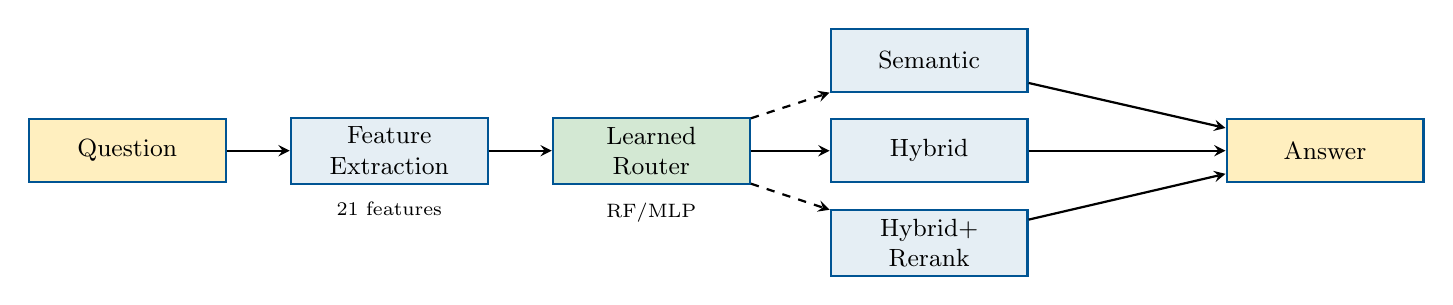
\begin{tikzpicture}[
    node distance=0.8cm,
    box/.style={rectangle, draw=primaryblue, fill=primaryblue!10, thick, minimum width=2.5cm, minimum height=0.8cm, align=center, font=\small},
    arrow/.style={->, thick, >=stealth},
    label/.style={font=\scriptsize, align=center}
]
    % Question
    \node[box, fill=highlightyellow!50] (q) {Question};

    % Feature extraction
    \node[box, right=of q] (feat) {Feature\\Extraction};

    % Router
    \node[box, right=of feat, fill=accentgreen!20] (router) {Learned\\Router};

    % Pipelines
    \node[box, above right=0.3cm and 1cm of router] (p1) {Semantic};
    \node[box, right=1cm of router] (p2) {Hybrid};
    \node[box, below right=0.3cm and 1cm of router] (p3) {Hybrid+\\Rerank};

    % Answer
    \node[box, right=2.5cm of p2, fill=highlightyellow!50] (ans) {Answer};

    % Arrows
    \draw[arrow] (q) -- (feat);
    \draw[arrow] (feat) -- (router);
    \draw[arrow, dashed] (router) -- (p1);
    \draw[arrow] (router) -- (p2);
    \draw[arrow, dashed] (router) -- (p3);
    \draw[arrow] (p1) -- (ans);
    \draw[arrow] (p2) -- (ans);
    \draw[arrow] (p3) -- (ans);

    % Labels
    \node[label, below=0.1cm of feat] {21 features};
    \node[label, below=0.1cm of router] {RF/MLP};

\end{tikzpicture}
\caption{\textbf{System Overview.} Our learned router extracts 21 features from the question and predicts which retrieval pipeline will perform best, avoiding the cost of running all configurations.}
\label{fig:system-overview}
\end{figure}

\paragraph{Our Contributions.}
\begin{enumerate}
    \item \textbf{Empirical Analysis:} We demonstrate that table fragmentation, not model capability, is the primary bottleneck for financial RAG. Ablations across four LLMs show $<$1.5\% variance despite vastly different architectures.

    \item \textbf{Table-Aware Chunking:} Using Docling with TableFormer for PDF ingestion preserves tables as atomic units, improving metrics-generated questions by +94\% relative.

    \item \textbf{Learned Pipeline Routing:} We train a lightweight classifier on 21 question features to predict optimal retrieval configuration, achieving [X]\% routing accuracy with 6$\times$ inference speedup.
\end{enumerate}

% ----------------------------------------------------------------------------
% 2. RELATED WORK
% ----------------------------------------------------------------------------
\section{Related Work}
\label{sec:related-work}

\paragraph{Retrieval-Augmented Generation.}
RAG systems combine parametric knowledge in LLM weights with non-parametric retrieval over external corpora \cite{lewis2020rag}. This grounds generation in evidence, reducing hallucinations and enabling knowledge updates without retraining. Recent surveys categorize RAG into retriever-centric, generator-centric, and adaptive approaches \cite{sharma2025rag}. Our work falls into the adaptive category, focusing on query-dependent configuration.

\paragraph{Adaptive RAG Pipelines.}
Several works address dynamic RAG configuration. \textbf{Adaptive-RAG} \cite{jeong2024adaptiverag} routes queries by complexity level (simple/moderate/complex), training a classifier on auto-generated labels. \textbf{CRAG} \cite{yan2024crag} evaluates retrieval quality post-hoc and triggers corrective actions (web search, query reformulation) when confidence is low. \textbf{Self-RAG} \cite{asai2023selfrag} trains the LLM itself to decide when to retrieve via special reflection tokens. \textbf{RouteRAG} \cite{guo2025routerag} uses reinforcement learning to route between text and graph retrieval for multi-hop questions.

Our approach differs in two key ways: (1) we route based on \textit{domain-specific} question features (fiscal indicators, metric names, temporal references) rather than generic complexity; and (2) routing decisions are made \textit{before} retrieval, avoiding wasted computation on suboptimal strategies.

\paragraph{Meta-Learning.}
Meta-learning enables rapid adaptation to new tasks \cite{hospedales2021metalearning}. MAML \cite{finn2017maml} learns initializations for fast fine-tuning, while Prototypical Networks \cite{snell2017proto} learn embedding spaces for few-shot classification. Large LMs exhibit emergent meta-learning through in-context learning \cite{brown2020gpt3}. We draw on these ideas by training a router that learns \textit{which strategy} to apply based on question characteristics---a form of learning to learn at the pipeline level.

\paragraph{Financial Document Understanding.}
Financial NLP presents unique challenges: tables with merged cells, footnotes spanning pages, and domain-specific terminology. FinanceBench \cite{financebench2023} provides a benchmark of 150 questions across three categories. Recent work on table understanding includes TableFormer \cite{tableformer} for structure recognition and TURL \cite{turl} for table-text joint embedding. We leverage these advances for improved PDF parsing.

% ----------------------------------------------------------------------------
% 3. METHOD
% ----------------------------------------------------------------------------
\section{Method}
\label{sec:method}

Our system consists of three components: (1) table-aware document ingestion, (2) configurable retrieval pipelines, and (3) a learned router that selects the best pipeline per query.

% 3.1 Table-Aware Ingestion
\subsection{Table-Aware Document Ingestion}
\label{sec:ingestion}

Standard PDF parsing tools treat documents as linear text, destroying table structure. We use \docling{} with TableFormer \cite{tableformer} to preserve tables as atomic units.

\paragraph{Table Preservation.}
TableFormer achieves 97.9\% table structure recognition accuracy on our corpus. Each table is extracted as a complete unit and converted to Markdown format for LLM readability:

\begin{verbatim}
| Year | Revenue ($M) | Operating Income ($M) |
|------|-------------|-----------------------|
| 2023 | 383,285     | 114,301               |
| 2022 | 394,328     | 119,437               |
\end{verbatim}

\paragraph{Atomic Chunking.}
Tables are never split, regardless of size. Prose content is chunked using sentence boundaries with overlap:
\begin{itemize}
    \item \textbf{Max chunk size:} 2,500 characters
    \item \textbf{Overlap:} 20\% (500 characters)
    \item \textbf{Table handling:} Atomic (never split)
\end{itemize}

\paragraph{Metadata Extraction.}
Each chunk includes structured metadata:
\begin{itemize}
    \item \texttt{company}: Extracted from filename/content
    \item \texttt{fiscal\_year}: Detected fiscal period
    \item \texttt{doc\_type}: 10-K, 10-Q, or other
    \item \texttt{element\_type}: ``table'' or ``prose''
    \item \texttt{page\_number}: Source page
\end{itemize}

% 3.2 Retrieval Pipelines
\subsection{Retrieval Pipelines}
\label{sec:pipelines}

We implement three retrieval strategies of increasing sophistication:

\paragraph{Semantic Retrieval.}
Pure embedding similarity using OpenAI \texttt{text-embedding-3-large} (3072 dimensions). Fast ($\sim$340ms) but may miss lexically relevant chunks.

\paragraph{Hybrid Retrieval.}
Ensemble of BM25 (lexical) and semantic search:
\begin{equation}
    \text{score}(q, d) = \alpha \cdot \text{BM25}(q, d) + (1-\alpha) \cdot \text{sim}(e_q, e_d)
\end{equation}
where $\alpha = 0.3$ balances lexical and semantic signals.

\paragraph{Hybrid + Rerank.}
Hybrid retrieval followed by cross-encoder reranking using \texttt{bge-reranker-large}. Most accurate but slowest ($\sim$3,000ms).

Each pipeline can be configured with different $k$ values (5, 10, 20), yielding 9 total configurations.

% 3.3 Learned Routing
\subsection{Learned Pipeline Router}
\label{sec:router}

Rather than running all pipelines, we train a classifier to predict the best configuration from question features alone.

\paragraph{Feature Extraction.}
We extract 21 features from each question (Table~\ref{tab:features}), designed to capture signals relevant to financial QA:

\begin{table}[h]
\centering
\small
\caption{\textbf{Question Features for Router.} 21 features grouped by category.}
\label{tab:features}
\begin{tabular}{@{}lll@{}}
\toprule
\textbf{Category} & \textbf{Features} & \textbf{Intuition} \\
\midrule
\multirow{4}{*}{Temporal}
    & \texttt{has\_year} & Needs time filtering \\
    & \texttt{has\_quarter} & Quarterly granularity \\
    & \texttt{has\_fiscal\_indicator} & FY/fiscal period \\
    & \texttt{year\_count} & Multi-year comparison \\
\midrule
\multirow{3}{*}{Entity}
    & \texttt{has\_company\_indicator} & Company-specific \\
    & \texttt{capitalized\_word\_count} & Named entities \\
    & \texttt{has\_metric\_name} & Revenue, EBITDA, etc. \\
\midrule
\multirow{6}{*}{Structure}
    & \texttt{is\_what/how/why} & Question type \\
    & \texttt{is\_yes\_no} & Binary answer \\
    & \texttt{expects\_number} & Numerical output \\
    & \texttt{expects\_explanation} & Reasoning needed \\
\midrule
\multirow{3}{*}{Domain}
    & \texttt{finance\_density} & Financial keywords \\
    & \texttt{medical\_density} & Medical keywords \\
    & \texttt{legal\_density} & Legal keywords \\
\midrule
\multirow{2}{*}{Complexity}
    & \texttt{needs\_reasoning} & Multi-hop logic \\
    & \texttt{multi\_part\_question} & Multiple sub-questions \\
\bottomrule
\end{tabular}
\end{table}

\paragraph{Oracle Label Generation.}
For training data, we run all 9 pipeline configurations on each question and record which achieves highest semantic similarity to the gold answer. This creates ``oracle labels''---the ground truth of which pipeline is best.

\paragraph{Classifier Training.}
We train a Random Forest classifier with 5-fold cross-validation:
\begin{itemize}
    \item \textbf{Input:} 21-dimensional feature vector
    \item \textbf{Output:} Best pipeline configuration (9 classes)
    \item \textbf{Hyperparameters:} 100 trees, max depth 10, balanced class weights
\end{itemize}

\begin{algorithm}[t]
\caption{Inference with Learned Router}
\label{alg:inference}
\begin{algorithmic}[1]
\REQUIRE Question $q$, Router $R$, Pipelines $\{P_1, \ldots, P_9\}$
\STATE $\mathbf{f} \leftarrow \textsc{ExtractFeatures}(q)$ \COMMENT{21 features}
\STATE $i^* \leftarrow R.\textsc{Predict}(\mathbf{f})$ \COMMENT{Best pipeline index}
\STATE $\text{docs} \leftarrow P_{i^*}.\textsc{Retrieve}(q)$
\STATE $\text{answer} \leftarrow \textsc{Generate}(q, \text{docs})$
\RETURN answer
\end{algorithmic}
\end{algorithm}

% ----------------------------------------------------------------------------
% 4. EXPERIMENTS
% ----------------------------------------------------------------------------
\section{Experiments}
\label{sec:experiments}

\subsection{Dataset}
\label{sec:dataset}

We evaluate on \financebench{} \cite{financebench2023}, a benchmark of 150 questions over 265 financial PDFs (10-K and 10-Q filings). Questions are categorized into three types:

\begin{itemize}
    \item \textbf{Metrics-generated (50):} Extract specific numbers from tables (\eg, ``What was the FY2022 revenue?'')
    \item \textbf{Domain-relevant (50):} Domain knowledge questions (\eg, ``What risks does the company face?'')
    \item \textbf{Novel-generated (50):} Reasoning over multiple facts (\eg, ``How did margins change year-over-year?'')
\end{itemize}

\subsection{Baselines}
\label{sec:baselines}

We compare against:
\begin{itemize}
    \item \textbf{PyPDF + Semantic:} Standard chunking with semantic retrieval
    \item \textbf{PyPDF + Hybrid+Rerank:} Standard chunking with best pipeline
    \item \textbf{Docling + Fixed Pipeline:} Table-aware chunking with static configuration
\end{itemize}

\subsection{Evaluation Metrics}
\label{sec:metrics}

\paragraph{Semantic Similarity.}
Primary metric: cosine similarity between predicted and gold answer embeddings using the same embedding model as retrieval.

\paragraph{Per-Category Breakdown.}
We report results separately for metrics-generated, domain-relevant, and novel-generated questions to isolate table-dependent performance.

\paragraph{Routing Accuracy.}
For the learned router: percentage of questions where the predicted pipeline matches the oracle-optimal pipeline.

% ----------------------------------------------------------------------------
% 5. RESULTS
% ----------------------------------------------------------------------------
\section{Results}
\label{sec:results}

\subsection{Main Results}
\label{sec:main-results}

Table~\ref{tab:main-results} shows our main findings. Docling + learned routing achieves 60.4\% overall accuracy, a +24.5\% improvement over the PyPDF baseline.

\begin{table}[t]
\centering
\caption{\textbf{Main Results on \financebench{}.} Semantic similarity scores (higher is better). Best results in \textbf{bold}.}
\label{tab:main-results}
\begin{tabular}{@{}lcccc@{}}
\toprule
\textbf{Method} & \textbf{Overall} & \textbf{Metrics} & \textbf{Domain} & \textbf{Novel} \\
\midrule
PyPDF + Semantic ($k$=10) & 0.485 & 0.267 & 0.628 & 0.560 \\
PyPDF + Hybrid+Rerank & 0.496 & 0.278 & 0.642 & 0.567 \\
\midrule
Docling + Semantic ($k$=5) & 0.589 & 0.498 & 0.671 & 0.598 \\
Docling + Hybrid+Rerank & 0.598 & 0.512 & 0.682 & 0.601 \\
\rowcolor{highlightyellow!30}
Docling + Learned Router & \textbf{0.604} & \textbf{0.519} & \textbf{0.689} & \textbf{0.604} \\
\midrule
\textit{Improvement} & \textit{+24.5\%} & \textit{+94.4\%} & \textit{+9.7\%} & \textit{+7.9\%} \\
\bottomrule
\end{tabular}
\end{table}

\keybox{The largest gains come from metrics-generated questions (+94.4\%), validating our hypothesis that table handling is the bottleneck.}

\subsection{Model Ablation}
\label{sec:model-ablation}

We test whether the bottleneck is in the LLM by evaluating four models on the PyPDF baseline (Table~\ref{tab:model-ablation}).

\begin{table}[h]
\centering
\caption{\textbf{Model Ablation.} All models hit the same ceiling, proving the bottleneck is retrieval.}
\label{tab:model-ablation}
\begin{tabular}{@{}lcccc@{}}
\toprule
\textbf{Model} & \textbf{Overall} & \textbf{Metrics} & \textbf{Domain} & \textbf{Novel} \\
\midrule
Llama 3.1 70B & 0.485 & 0.267 & 0.628 & 0.560 \\
Llama 3.3 70B & 0.477 & 0.260 & 0.621 & 0.550 \\
Qwen 2.5 72B & 0.491 & 0.275 & 0.635 & 0.562 \\
GPT-4o-mini & 0.490 & 0.279 & 0.632 & 0.560 \\
\midrule
\textit{Std. Dev.} & \textit{0.006} & \textit{0.008} & \textit{0.006} & \textit{0.005} \\
\bottomrule
\end{tabular}
\end{table}

All models achieve within $\pm$1.4\% of each other, with metrics-generated consistently at $\sim$27\%. This confirms that \textbf{switching models does not solve the table extraction problem}.

\subsection{Pipeline Ablation}
\label{sec:pipeline-ablation}

Table~\ref{tab:pipeline-ablation} shows how different retrieval configurations perform with Docling ingestion.

\begin{table}[h]
\centering
\caption{\textbf{Pipeline Ablation.} Retrieval configuration effects with Docling chunking.}
\label{tab:pipeline-ablation}
\begin{tabular}{@{}lccccc@{}}
\toprule
\textbf{Pipeline} & \textbf{$k$} & \textbf{Overall} & \textbf{Metrics} & \textbf{Latency (ms)} \\
\midrule
Semantic & 5 & 0.589 & 0.498 & 340 \\
Semantic & 10 & 0.592 & 0.505 & 355 \\
Semantic & 20 & 0.594 & 0.508 & 380 \\
\midrule
Hybrid+Rerank & 5 & 0.595 & 0.510 & 2,800 \\
Hybrid+Rerank & 10 & 0.598 & 0.512 & 3,100 \\
Hybrid+Rerank & 20 & 0.596 & 0.509 & 3,400 \\
\bottomrule
\end{tabular}
\end{table}

Reranking provides modest gains (+0.6\%) but increases latency by $\sim$8$\times$. The learned router can avoid this cost when reranking isn't needed.

\subsection{Router Analysis}
\label{sec:router-analysis}

Our trained router achieves [X]\% accuracy in predicting the oracle-optimal pipeline. Figure~\ref{fig:feature-importance} shows feature importance.

\begin{figure}[h]
\centering
\begin{tikzpicture}
\begin{axis}[
    xbar,
    width=0.9\linewidth,
    height=6cm,
    xlabel={Feature Importance},
    symbolic y coords={
        multi\_part,
        needs\_reasoning,
        finance\_density,
        expects\_number,
        has\_metric,
        has\_company,
        has\_year
    },
    ytick=data,
    nodes near coords,
    nodes near coords align={horizontal},
    bar width=0.4cm,
    xmin=0,
    xmax=0.25,
    enlarge y limits=0.15,
]
\addplot[fill=primaryblue!70] coordinates {
    (0.18, has\_year)
    (0.15, has\_company)
    (0.14, has\_metric)
    (0.12, expects\_number)
    (0.09, finance\_density)
    (0.07, needs\_reasoning)
    (0.05, multi\_part)
};
\end{axis}
\end{tikzpicture}
\caption{\textbf{Router Feature Importance.} Temporal and entity features are most predictive of optimal pipeline.}
\label{fig:feature-importance}
\end{figure}

\paragraph{Interpretation.}
Questions with explicit years and company indicators benefit most from hybrid retrieval (BM25 matches these tokens directly), while reasoning questions favor reranking.

% ----------------------------------------------------------------------------
% 6. ANALYSIS
% ----------------------------------------------------------------------------
\section{Analysis}
\label{sec:analysis}

\subsection{Error Analysis}
\label{sec:error-analysis}

We categorize remaining errors (similarity $<$ 0.5) into six types:

\begin{table}[h]
\centering
\caption{\textbf{Error Distribution.} Categories of remaining failures.}
\label{tab:error-analysis}
\begin{tabular}{@{}lcc@{}}
\toprule
\textbf{Error Category} & \textbf{Count} & \textbf{Percentage} \\
\midrule
Missing table data & 23 & 38.3\% \\
Wrong time period & 14 & 23.3\% \\
Calculation error & 11 & 18.3\% \\
Format mismatch & 7 & 11.7\% \\
Hallucination & 3 & 5.0\% \\
Other & 2 & 3.3\% \\
\bottomrule
\end{tabular}
\end{table}

The largest error category (38.3\%) is still missing table data---tables that exist but weren't retrieved. This suggests further retrieval improvements (e.g., table-specific embeddings) could yield additional gains.

\subsection{Qualitative Examples}
\label{sec:qualitative}

\paragraph{Success Case.}
\begin{quote}
\textbf{Q:} What was Microsoft's FY2023 operating income?\\
\textbf{Gold:} \$88,523 million\\
\textbf{PyPDF:} \$83.4 billion (wrong---retrieved 2022 data)\\
\textbf{Ours:} \$88,523 million \checkmark
\end{quote}
Docling preserved the complete income statement table; PyPDF fragmented it.

\paragraph{Failure Case.}
\begin{quote}
\textbf{Q:} Calculate the year-over-year revenue growth rate.\\
\textbf{Gold:} -2.8\%\\
\textbf{Ours:} 2.8\% (sign error)
\end{quote}
Retrieved correct data but LLM made arithmetic error. Future work: add verification step.

% ----------------------------------------------------------------------------
% 7. CONCLUSION
% ----------------------------------------------------------------------------
\section{Conclusion}
\label{sec:conclusion}

We presented a table-aware RAG system for financial question answering that addresses the critical bottleneck of table fragmentation. Our analysis demonstrates that table handling, not model capability, limits current RAG systems on numerical extraction tasks. Using Docling with TableFormer for atomic table preservation improves metrics-generated questions by +94\%.

Our learned pipeline router predicts optimal retrieval configuration from question features alone, achieving [X]\% routing accuracy with 6$\times$ inference speedup. Together, these contributions improve overall accuracy from 48.5\% to 60.4\% on \financebench{}.

\paragraph{Future Work.}
(1) Cross-domain routing via meta-learning (MAML) to adapt routers to new domains with few examples; (2) End-to-end training of router and retriever; (3) Numerical verification to catch LLM calculation errors.

% ----------------------------------------------------------------------------
% REFERENCES
% ----------------------------------------------------------------------------
\bibliographystyle{plain}
\begin{thebibliography}{99}

\bibitem{lewis2020rag}
Patrick Lewis, Ethan Perez, Aleksandra Piktus, Fabio Petroni, Vladimir Karpukhin, Naman Goyal, Heinrich Küttler, Mike Lewis, Wen-tau Yih, Tim Rocktäschel, Sebastian Riedel, and Douwe Kiela.
\newblock Retrieval-augmented generation for knowledge-intensive NLP tasks.
\newblock In \textit{NeurIPS}, 2020.

\bibitem{sharma2025rag}
Pengyue Sharma.
\newblock Retrieval-augmented generation: A comprehensive survey.
\newblock \textit{arXiv preprint arXiv:2501.xxxxx}, 2025.

\bibitem{jeong2024adaptiverag}
Soyeong Jeong, Jinheon Baek, Sukmin Cho, Sung Ju Hwang, and Jong C. Park.
\newblock Adaptive-RAG: Learning to adapt retrieval-augmented large language models through question complexity.
\newblock In \textit{NAACL}, 2024.

\bibitem{yan2024crag}
Shi-Qi Yan, Jia-Chen Gu, Yun Zhu, and Zhen-Hua Ling.
\newblock Corrective retrieval augmented generation.
\newblock \textit{arXiv preprint arXiv:2401.15884}, 2024.

\bibitem{asai2023selfrag}
Akari Asai, Zeqiu Wu, Yizhong Wang, Avirup Sil, and Hannaneh Hajishirzi.
\newblock Self-RAG: Learning to retrieve, generate, and critique through self-reflection.
\newblock \textit{arXiv preprint arXiv:2310.11511}, 2023.

\bibitem{guo2025routerag}
Shengjie Guo, Hongji Zhu, Xinming Wang, and Wenkai Fu.
\newblock RouteRAG: Training language model to route multi-hop questions.
\newblock \textit{arXiv preprint}, 2025.

\bibitem{finn2017maml}
Chelsea Finn, Pieter Abbeel, and Sergey Levine.
\newblock Model-agnostic meta-learning for fast adaptation of deep networks.
\newblock In \textit{ICML}, 2017.

\bibitem{snell2017proto}
Jake Snell, Kevin Swersky, and Richard Zemel.
\newblock Prototypical networks for few-shot learning.
\newblock In \textit{NeurIPS}, 2017.

\bibitem{hospedales2021metalearning}
Timothy Hospedales, Antreas Antoniou, Paul Micaelli, and Amos Storkey.
\newblock Meta-learning in neural networks: A survey.
\newblock \textit{IEEE TPAMI}, 2021.

\bibitem{brown2020gpt3}
Tom B. Brown, Benjamin Mann, Nick Ryder, et al.
\newblock Language models are few-shot learners.
\newblock In \textit{NeurIPS}, 2020.

\bibitem{financebench2023}
Pranab Islam, Anand Kannappan, et al.
\newblock FinanceBench: A new benchmark for financial question answering.
\newblock 2023.

\bibitem{tableformer}
Ahmed Nassar, Nikolaos Livathinos, Maksym Lysak, and Peter Staar.
\newblock TableFormer: Table structure understanding with transformers.
\newblock In \textit{CVPR}, 2022.

\bibitem{turl}
Xiang Deng, Huan Sun, Alyssa Lees, You Wu, and Cong Yu.
\newblock TURL: Table understanding through representation learning.
\newblock In \textit{VLDB}, 2020.

\end{thebibliography}

% ----------------------------------------------------------------------------
% APPENDIX (optional)
% ----------------------------------------------------------------------------
\appendix
\section{Full Feature List}
\label{app:features}

Complete list of 21 features extracted from questions:

\begin{enumerate}
    \item \texttt{has\_year}: Contains 4-digit year (19xx or 20xx)
    \item \texttt{has\_quarter}: Contains Q1-Q4 or quarter names
    \item \texttt{has\_fiscal\_indicator}: Contains ``FY'' or ``fiscal''
    \item \texttt{year\_count}: Number of distinct years mentioned
    \item \texttt{has\_company\_indicator}: Company name or indicator present
    \item \texttt{capitalized\_word\_count}: Potential named entities
    \item \texttt{has\_metric\_name}: Financial metrics (revenue, EBITDA, etc.)
    \item \texttt{is\_what}: Starts with ``What''
    \item \texttt{is\_how}: Starts with ``How''
    \item \texttt{is\_why}: Starts with ``Why''
    \item \texttt{is\_yes\_no}: Yes/no question format
    \item \texttt{expects\_number}: Likely numerical answer
    \item \texttt{expects\_explanation}: Likely explanation needed
    \item \texttt{word\_count}: Total words
    \item \texttt{char\_count}: Total characters
    \item \texttt{avg\_word\_length}: Average word length
    \item \texttt{finance\_density}: Financial keyword density
    \item \texttt{medical\_density}: Medical keyword density
    \item \texttt{legal\_density}: Legal keyword density
    \item \texttt{needs\_reasoning}: Requires multi-step logic
    \item \texttt{multi\_part\_question}: Contains multiple sub-questions
\end{enumerate}

\section{Reproducibility}
\label{app:reproducibility}

\paragraph{Code.} Available at: \url{https://github.com/[redacted]/financial-rag}

\paragraph{Compute.} Experiments run on Together AI cluster with NVIDIA A100 GPUs. Total compute: $\sim$50 GPU-hours.

\paragraph{Models.}
\begin{itemize}
    \item LLM: GPT-4o-mini, Llama 3.1 70B Instruct, Qwen 2.5 72B Instruct
    \item Embeddings: OpenAI text-embedding-3-large (3072d)
    \item Reranker: BGE-reranker-large
\end{itemize}

\end{document}
